\chapter{Experimentální část}
Experimentální studii suspendace v mechanicky míchané nádobě provedla Bc.\,Zuzana Pavlíková v rámci své bakalářské práce na Ústavu chemického inženýrství VŠCHT Praha v roce 2011.

\section{Popis experimentu}
\label{chap:exp}
Náplní experimentu bylo měření průběhu homogenizace kapaliny v přítomnosti pevné fáze a následném zjišťování doby homogenizace. K provedení experimentu byla využita válcová nádoba z plexiskla o vnitřním průměru $T=\SI{0.29}{\meter}$ s plochým dnem, jenž byla opatřena čtyřmi radiálními narážkami o šířce $b=T/10$. Výška plnění nádoby byla zvolena $H=T$. 

\begin{figure}[h!]
\begin{center}
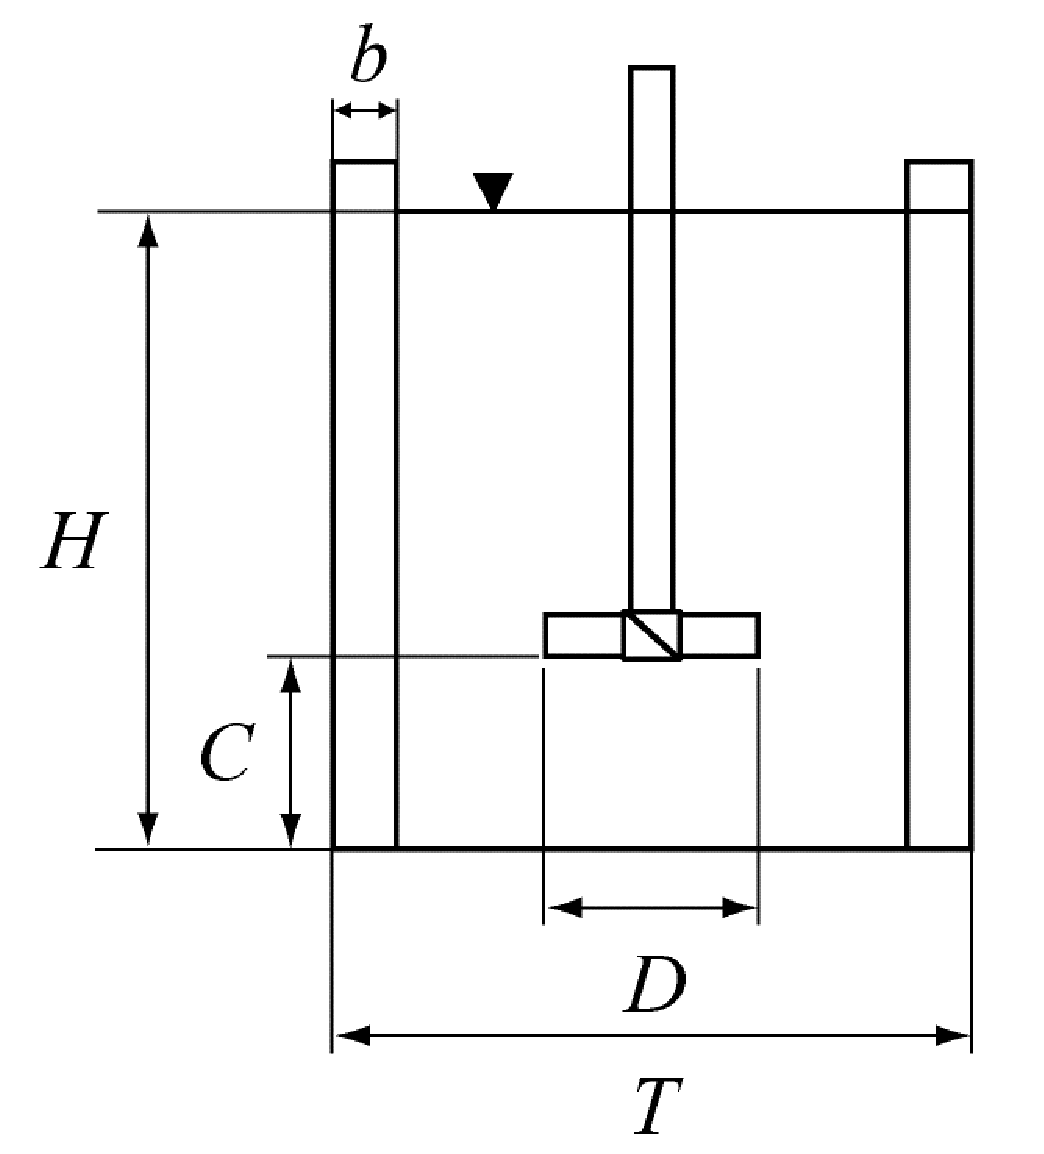
\includegraphics[scale=0.45]{images/mujedit.eps}
\caption{Geometrie experimentu}
\label{fig:nadoba}
\end{center}
\end{figure} 

Do nádoby $C=T/3$ ode dna bylo umístěno šestilopatkové míchadlo se šikmo skloněnými lopatkami (úhel zkosení \SI{45}{\degree}). Rychlost otáčení byla postupně volena  \SIlist[list-units = single]{3;4;5;6;7;8;9}{\per\second}. Celkový průměr míchadla činil $D=T/3$ a ostatní jeho rozměry jsou zobrazuje obr. XX.      

Jako vsádka byla použita voda a polyvinylpyrrolidon (PVP). Pevnou fázi tvořily červené kuličky z polyvinylchloridu (PVC) o průměru \SI{1.02}{\milli\meter}. Vsádka postupně obsahovala 5, 10 a 15\,\%\,obj. těchto kuliček. Vlastnosti kapalné a pevné fáze jsou shrnuty v tab. \ref{tab:fyzvlast}. 


\begin{table}[h!]
\begin{center}
		\caption{Stanovené vlastnosti kapalné a pevné fáze}
		\label{tab:fyzvlast}
\begin{tabular}{|c|S[table-parse-only]|s|}
  
\hline
  
{\textbf{Veličina}} & {\textbf{Hodnota}} & {\textbf{Jednotka}} \\ \hline
hustota vody & 999.50 & \kilogram\per\cubic\meter \\ \hline{}
hustota PVP\,5 & 1011.44 & \kilogram\per\cubic\meter \\ \hline{}
hustota PVP\,7.5 & 1024.18 & \kilogram\per\cubic\meter \\ \hline{}
hustota kuliček z PVC & 1136.0 & \kilogram\per\cubic\meter \\ \hline{}
průměr kuliček z PVC & 1.02 & \milli\meter \\ \hline{}
mezerovitost kuliček z PVC & 0.384 & -- \\ \hline{}
dynamická viskozita vody & 1.138 & \milli\pascal\second \\ \hline
dynamická viskozita PVP\,5 & 5.050 & \milli\pascal\second \\ \hline{}
dynamická viskozita PVP\,7.5 & 7.615 & \milli\pascal\second \\ \hline

\end{tabular}
\end{center}
\end{table}

K měření doby homogenizace byla využita vodivostní metoda při které je do nádoby ponoře sonda snímající okamžitou hodnotu napětí. Zjištěná hodnota napětí byla  následně přepočítána na bezrozměrnou koncentraci $c^{*}(t)$ podle rovnice \ref{eq:bezkonc}, kde $c(t)$ a $U(t)$ je koncentrace respektive napětí v daném čase $t$.   

\begin{equation}
	c^{*}(t) = \frac{c(t) - c(0)}{c(\infty) - c(0)} \approx \frac{U(t) - U(0)}{U(\infty) - U(0)}
	\label{eq:bezkonc}
\end{equation}

Na počátku experimentu byla do nádoby nadávkována indikační látka (NaCl) a sledována hodnota její koncentrace respektive napětí. Doba po které dosáhla fluktuace bezrozměrné koncentrace hodnoty menší než \SI{5}{\percent}, byla považována za dobu homogenizace. 





